\documentclass[conf]{new-aiaa}
\usepackage[utf8]{inputenc}

\usepackage{graphicx}
\usepackage{amsmath}
\usepackage{siunitx}
\usepackage{float}
\usepackage{longtable,tabularx}
\usepackage{multirow, multicol}
\usepackage{minted}
\usepackage{verbatim}
\usepackage[ruled,vlined]{algorithm2e}

\usepackage{geometry}
\geometry{margin=0.86in}

% From https://tex.stackexchange.com/questions/323297/
\newcommand{\rvline}{\hspace*{-\arraycolsep}\vline\hspace*{-\arraycolsep}}

\graphicspath{{./media/}}

\usepackage{hyperref}
\renewcommand\refname{}
\urlstyle{same}
\hypersetup{
    colorlinks=false,
    linkcolor=black,
    filecolor=black,      
    urlcolor=cyan,
}

\title{Exploring Invariant Manifolds for Low-Cost Trajectory Design}

\author{Joseph D. Carpinelli
    \footnote{
        Graduate Assistant, 
        Department of Aerospace Engineering, 
        University of Maryland, College Park}}
\affil{DRAFT -- Extended Abstract \\ \today}

\begin{document}

\maketitle

\begin{abstract}
    Periodic orbits within the Circular Restricted Three-body Problem 
    (CR3BP) are more difficult to find than periodic orbits within the 
    Restricted Two-body Problem (R2BP). While any  elliptical or circular 
    R2BP orbit is periodic, the periodic subset of CR3BP orbits is far 
    more selective. Periodic CR3BP orbit-finding algorithms 
    have been known for decades, but their implementations are not easily
    found in free and open-source software -- the few implementations
    which do exist in free and open-source software don't hold 
    \textit{generally}. Instead, publicly accessible implementations may 
    find periodic orbits for one particular CR3BP system (e.g. Sun-Earth), 
    or  may find periodic orbits which have non-zero z-amplitudes. 
    General solutions for periodic CR3BP orbits are incredibly useful, as 
    CR3BP analysis is often used as an approximate starting-point in 
    mission design. In addition, invariant manifolds about periodic 
    CR3BP orbits can provide low-cost interplanetary transfers when 
    compared with traditional transfer designs. This paper introduces 
    a matured periodic CR3BP orbit-finding implementation that works 
    \textit{generally}. This implementation is used to highlight several
    Halo orbit families in familiar CR3BP systems, calculate invariant 
    manifolds about Halo orbits, and use the invariant manifolds to 
    calculate low-cost interplanetary transfer designs. A CR3BP 
    patched-conic mission design will be presented. All source code 
    is available on GitHub as part of 
    \textit{UnitfulAstrodynamics.jl}, an astrodynamics package written 
    with Julia.

\end{abstract}

\begin{multicols*}{2}

\section*{Contents}
A TOC is \textit{not} included in this draft 
to help save space for actual content. 
Read on for some fun orbit plots!
% \tableofcontents

\section{Nomenclature}
\begin{flushleft}
\begin{tabularx}{\columnwidth}{ccl}
    $\overrightarrow{r}$ & $=$ & Spacecraft position \\
    $\overrightarrow{v}$ & $=$ & Spacecraft velocity \\
    $\Phi_m$             & $=$ & Monodromy matrix \\
    $\Phi$               & $=$ & State transition matrix \\
    R2BP                 & $=$ & Restricted Two-body Problem \\
    CR3BP                & $=$ & Circular Restricted Three-body Problem \\
    $S_L \triangleq a$   & $=$ & Distance between CR3BP bodies \\
    $S_T$                & $=$ & Time scale factor \\
    $\mu^\star$ & $=$    & Normalized CR3BP mass parameter \\
    $\overrightarrow{r}^\star$ & $=$ & Normalized spacecraft position \\
    $\overrightarrow{v}^\star$ & $=$ & Normalized spacecraft velocity \\
    $r_i$                & $=$ & Nondimensional $x$ position of $i_{\text{th}}$ body \\ 
\end{tabularx}
\end{flushleft}

\section{Introduction}
As space exploration targets shift from Earth's moon to Mars and 
beyond, low-cost trajectory designs are increasingly important 
\cite{nasa2020artemis}. One such family of low-cost trajectory 
designs utilizes invariant manifolds about Lagrange points
\cite{rund2018interplanetary}. Halo orbits can be estimated 
analytically with an expansion, as originally shown by Richardson 
\cite{richardson1980analytical} \cite{koon2008dynamical}. A known
numerical algorithm can iterate on non-periodic initial Halo orbit 
conditions to produce numerically periodic Halo orbits
\cite{howell1984three}. When placed in series, these two algorithms 
provide a proverbial \textit{black box} for astrodynamicists: 
given desired physical features (orbit amplitude, phase, etc.), 
the analytical algorithm can produce a Halo orbit estimate for the
numerical algorithm to iterate on \cite{rund2018interplanetary}.
These algorithms were recently implemented with the Julia 
programming language \cite{carpinelli2020halos} 
\cite{carpinelli2020astro} \cite{bezanson2017julia}. 

This paper presents low-cost manifold-based trajectories from 
the Sun-Earth system, to Sun-Mars and Sun-Jupiter systems. 
Manifold and traditional trajectory designs will be compared, 
and their costs and benefits will be analyzed. 

First, an overview of the Circular Restricted Three-body Problem,
and periodic CR3BP orbits, is provided. Methods for calculating
periodic CR3BP orbits are briefly discussed, and a Julia 
implementation is introduced. Test cases are presented for 
the analytical and numerical Halo orbit solvers 
\cite{carpinelli2020halos}. 
These test cases will help to guarantee that the Julia 
Halo solvers within UnitfulAstrodynamics.jl are working correctly,
and they may serve as a helpful troubleshooting resource 
for others who hope to implement similar algorithims 
\cite{carpinelli2020astro}. 

Next, a short catalog of Sun-Earth, Sun-Mars, and Sun-Jupiter 
Halo orbits is presented using the developed Halo solvers.
This catalog will provide parameters for each Halo orbit, 
and initial conditions and orbital periods from which to propagate.

Visualizations for stable and unstable 
manifolds near each chosen Halo orbit are shown. Points along the 
Halo orbits' stable manifolds are found, and 
transfers between LEO and these stable manifolds are defined. 
These manifolds are then used to generate interplanetary 
transfers. The manifold-based transfers will be compared and 
contrasted against traditional transfer designs (e.g. Hohmann, 
Lambert). The following analysis metrics are addressed: total 
mission $\Delta v$, total mission duration, and (ideal) 
number of maneuvers.

All code written for this project is included in the open-source 
Julia package titled \textit{UnitfulAstrodynamics.jl} \cite{carpinelli2020astro}.
A Pluto (Jupyter-like) notebook with code examples, and an informal 
project summary is provided 
\cite{fosnp2020Pluto} \cite{carpinelli2020halos}.

\section{Technical Overview}

\subsection{CR3BP Overview}
The Circular Restricted Three-body Problem is a simplified 
dynamical model of an infinitesimally small spacecraft traveling
near two finite-mass celestial bodies. All masses are described
as point masses. The system's barycenter is the 
center of mass of the two celestial bodies, and both celestial 
bodies are constrained to travel in a circle about an inertial 
frame placed at the system barycenter. CR3BP spacecraft dynamics are 
typically described in the \textit{Synodic} frame, which is placed
at the barycenter of the system, and rotates about its Z axis such 
that each celestial body is fixed on the Synodic X axis. 
CR3BP spacecraft dynamics are also typically described with 
normalized units,
as shown in equations $\left(1\right)$ $\left(2\right)$ $\left(3\right)$
$\left(4\right)$. Normalized equations of motion for a spacecraft 
within the CR3BP are shown in equations 
$\left(5\right)$ $\left(6\right)$ $\left(7\right)$ $\left(8\right)$
$\left(9\right)$. Note that $\mu_2 < \mu_1$.

\textit{
    Relevant CR3BP definitions, calculations, and 
    equations of motion will be presented here.
}

\begin{comment}
\subsubsection*{Normalized Synodic CR3BP State}
\begin{align}
    \mu^\star & = \frac{\mu_2}{\mu_1+\mu_2} \\
    S_t & = \sqrt{\frac{a^3}{\mu_1+\mu_2}} \\
    \overrightarrow{r}^\star & \triangleq \begin{bmatrix} x^\star & y^\star & z^\star \end{bmatrix}^T  = \frac{1}{S_L} \overrightarrow{r} \\
    \overrightarrow{v}^\star & \triangleq \begin{bmatrix} \dot{x}^\star & \dot{y}^\star & \dot{z}^\star \end{bmatrix}^T  = \frac{1}{S_T} \overrightarrow{v}
\end{align}

\subsubsection*{Normalized Synodic CR3BP Dynamics}

\begin{align}
    r_1 & = \sqrt{(x^\star+\mu^\star)^2 + (y^\star)^2 + (z^\star)^2} \\
    r_2 & = \sqrt{(x^\star+\mu^\star-1)^2 + (y^\star)^2 + (z^\star)^2} \\
    \ddot{x}^\star & = 2\dot{y}^\star + x^\star - \frac{(1-\mu^\star)(x^\star + \mu^\star)}{r_1^3} - 
        \frac{\mu^\star (x^\star - 1 + \mu^\star)}{r_2^3} \\
    \ddot{y}^\star & = -2\dot{x}^\star + y^\star - \frac{(1 - \mu^\star)y^\star}{r_1^3} - \frac{\mu^\star y^\star}{r_2^3} \\
    \ddot{z}^\star & = -\frac{(1-\mu^\star)z^\star}{r_1^3} - \frac{\mu^\star z^\star}{r_2^3}
\end{align}

\end{comment}
\subsection{Periodic CR3BP Orbits}

Planar periodic CR3BP orbits about the first or second Lagrange point
(L1 or L2) are known as Lypunov orbits, while periodic CR3BP orbits
about L1 or L2 with non-zero Z components are known as Halo orbits 
\cite{koon2008dynamical}.
Periodic CR3BP orbits are desirable for many reasons, including
eclipse avoidance 
\cite{williams2017targeting}.
Of course, orbits within the CR3BP are \textbf{not} guaranteed to be
periodic. An estimated analytical periodic orbit solution can be found 
with a third-order expansion, as originally shown by Dr. Richardson
\cite{richardson1980analytical}
\cite{koon2008dynamical}
\cite{rund2018interplanetary}. 
Dr. Howell developed an iterative algorithm find a numerically 
periodic CR3BP orbit
\cite{howell1984three} 
\cite{koon2008dynamical} 
\cite{rund2018interplanetary}.
The analytical and iterative periodic orbit-finding algorithms 
are described in more detail in the remainder of this section.

\subsubsection{Analytical Solution}
Approximate analytical solutions exist for periodic orbits within
the Circular Restricted Three-body Problem. CR3BP dynamics can 
be written as a polynomial expansion 
\cite{koon2008dynamical}. 
Dr. Richardson used a third-order expansion to develop an 
analytical solution for periodic CR3BP orbits about L1 or L2;
the solution involves changing coordinates to be centered 
at the desired Lagrange point and normalized to the 
distance between the lagrange point and the less-massive 
celestial body 
\cite{koon2008dynamical} 
\cite{richardson1980analytical}
\cite{rund2018interplanetary}.
This analytical solution is described in far more detail 
by Rund and Koon et al 
\cite{rund2018interplanetary} 
\cite{koon2008dynamical}.
Here, the reader should know two important points 
about this analytical method: each periodic orbit 
can be completely described by its Z amplitude 
(as a result of a X and Z amplitude constraint), 
and because each analytical solution is only 
an \textit{approximation}, propagating any 
analytical result does \textit{not} result 
in a numerically periodic orbit
\cite{koon2008dynamical}.
The latter point is shown by \figurename{1}.

\vskip -0.3cm
\begin{figure}[H]
    \hskip -0.3cm
    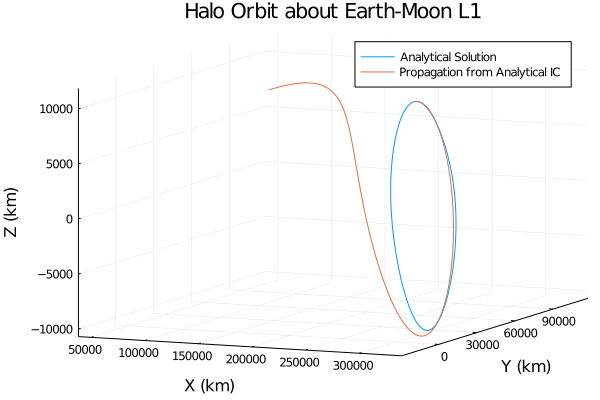
\includegraphics[width=0.5\textwidth]{analytical_propagation.png}
    \caption{Numerically propagated analytical solution}
\end{figure}

\subsubsection{Numerical Solution}

\textit{
    A description of the iterative Halo orbit-finding 
    algorithm will be provided here. The description 
    will be at a somewhat high level, similar to the 
    analytical solution description above. Still,
    the \textbf{algorithm} package will be used to outline
    the numerical algorithm, and a Julia implementation
    will be briefly presented. The plots below 
    will be shown in the final paper: the first 
    shows how the numerical algorithm iterates on 
    a periodic orbit candidate produced by the 
    analytical solution, and the second
    shows a family of periodic CR3BP orbits 
    that were produced by the Julia implementation.
}

\begin{figure}[H]
    \hskip -0.3cm
    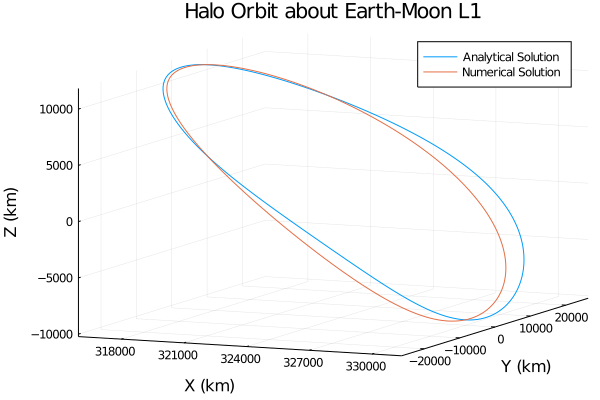
\includegraphics[width=0.5\textwidth]{analytical_numerical_halo.png}
    \caption{Analytical and Iterative Numerical solutions}
\end{figure}

\begin{figure}[H]
    \hskip -0.3cm
    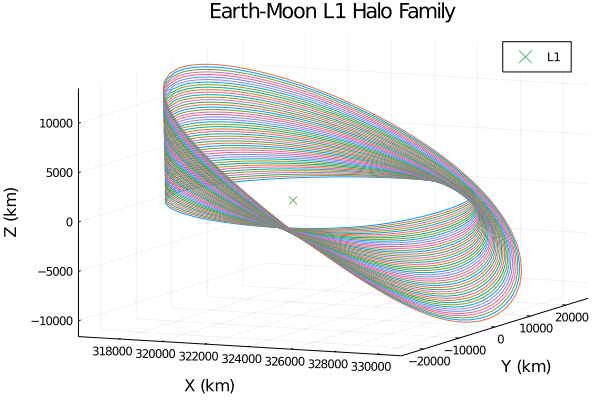
\includegraphics[width=0.5\textwidth]{halo_family_example.png}
    \caption{Famly of Halo orbits about Earth-Moon L1}
\end{figure}

\subsection{Invariant Manifolds}

\textit{
    The mathematics behind invariant manifolds will be 
    presented. An invariant manifold-finding algorithm 
    will be presented, as shown by Rund and Koon et al 
    \cite{rund2018interplanetary}
    \cite{koon2008dynamical}.
    Stable and unstable invariant manifolds near Halo 
    orbits will be shown, as produced by a Julia 
    implementation of the previously mentioned 
    algorithm.
}

\subsection{Manifold-based Transfers}

\textit{
    An algorithm for using invariant manifolds to 
    design interplanetary transfers will be presented,
    as summarized by Rund \cite{rund2018interplanetary}.
    A Julia implementation will (hopefully!) be presented
    here as well.
}

\section{Results}

\subsection{Numerically Periodic CR3BP Orbits}

\textit{
    A large table (1-2 pages) of autogenerated periodic
    orbits about Lagrange points of familiar 
    CR3BP systems will be provided here. I'll write 
    some code to find several families of Halo orbits 
    about the Sun-Earth, Earth-Moon, Sun-Mars, and 
    Sun-Jupiter systems. This will hopefully be a 
    helpful reference for future astrodynamics students.
}

\subsection{Transfer Design Comparisons}

\textit{
    A table (half a page) of Hohmann, Lambert, 
    and manifold-based transfer designs from 
    Earth to Mars and Jupiter will be presented. 
    The results will be discussed, including
    cost and time duration comparisons between
    transfer designs. If there is time, a GMAT-like 
    tool will also be presented. This tool 
    will allow for user inputs, such as 
    "start at Earth, transfer to Jupiter, 
    end at 7000 km Z amplitude orbit 
    about Io."
}

\section{Conclusion}

\section{References}
\nocite{*}
\renewcommand\refname{\vskip -0.9cm}
\bibliography{sources}

\section{Appendix}
\textit{
    Will present all source code necessary to replicate 
    this project, including copy-pasted UnitfulAstrodynamics.jl
    code that is available on GitHub. Any MATLAB implementations 
    will also be provided here, as MATLAB is a far more common 
    tool used by astrodynamics students. 
}

\end{multicols*}

\end{document}